\documentclass[Crown,sageh,times]{sagej}
\usepackage{moreverb,url}
%\usepackage[bookmarksopen,bookmarksnumbered,citecolor=black,urlcolor=black]{hyperref}
\newcommand\BibTeX{{\rmfamily B\kern-.05em \textsc{i\kern-.025em b}\kern-.08em
T\kern-.1667em\lower.7ex\hbox{E}\kern-.125emX}}
\def\volumeyear{2017}

\RequirePackage[citecolor=0 0 0,colorlinks=false]{hyperref}
\hypersetup{
     breaklinks=true,
     bookmarksopen=true,
     bookmarksnumbered=true,
     linkcolor=black,
     urlcolor=black,
     citecolor=black,
     colorlinks=true}


%%% The amssymb package provides various useful mathematical symbols
%\usepackage{amssymb}
%%% The amsthm package provides extended theorem environments
% \usepackage{amsthm}
% \usepackage{amsmath}
% \usepackage{color}
% \usepackage{amsmath}
%\usepackage{siunitx}
%\usepackage{framed} % Framing content
%\usepackage{multicol} % Multiple columns environment
%\usepackage{nomencl} % Nomenclature package
%\makenomenclature
%%\setlength{\nomitemsep}{-\parskip} % Baseline skip between items
%\setlength{\nomitemsep}{0.01cm}
%\renewcommand*\nompreamble{\begin{multicols}{2}}
%\renewcommand*\nompostamble{\end{multicols}}
%\newcommand{\degreeC}{\ensuremath{^\circ}C }
\usepackage{eurosym}
\usepackage{booktabs}

\usepackage{todonotes}


\begin{document}

\runninghead{The `Paris-end' of town? Urban typology through machine learning. Supplemental Material}
\title{The `Paris-end' of town? Urban typology through machine learning.}



\maketitle


\begin{figure}[!htbp]
\centering 
\includegraphics[scale=0.4]{Images/MelbourneEvaluationLocations.png}   
\includegraphics[scale=0.4]{Images/SydneyEvaluationLocations.png}    
\caption{\bf Evaluation locations for Melbourne (left) and Sydney (right).}    
 \label{fig:supp_melsydevallocations}  
\end{figure} 

\begin{figure}[!htbp]
\centering     
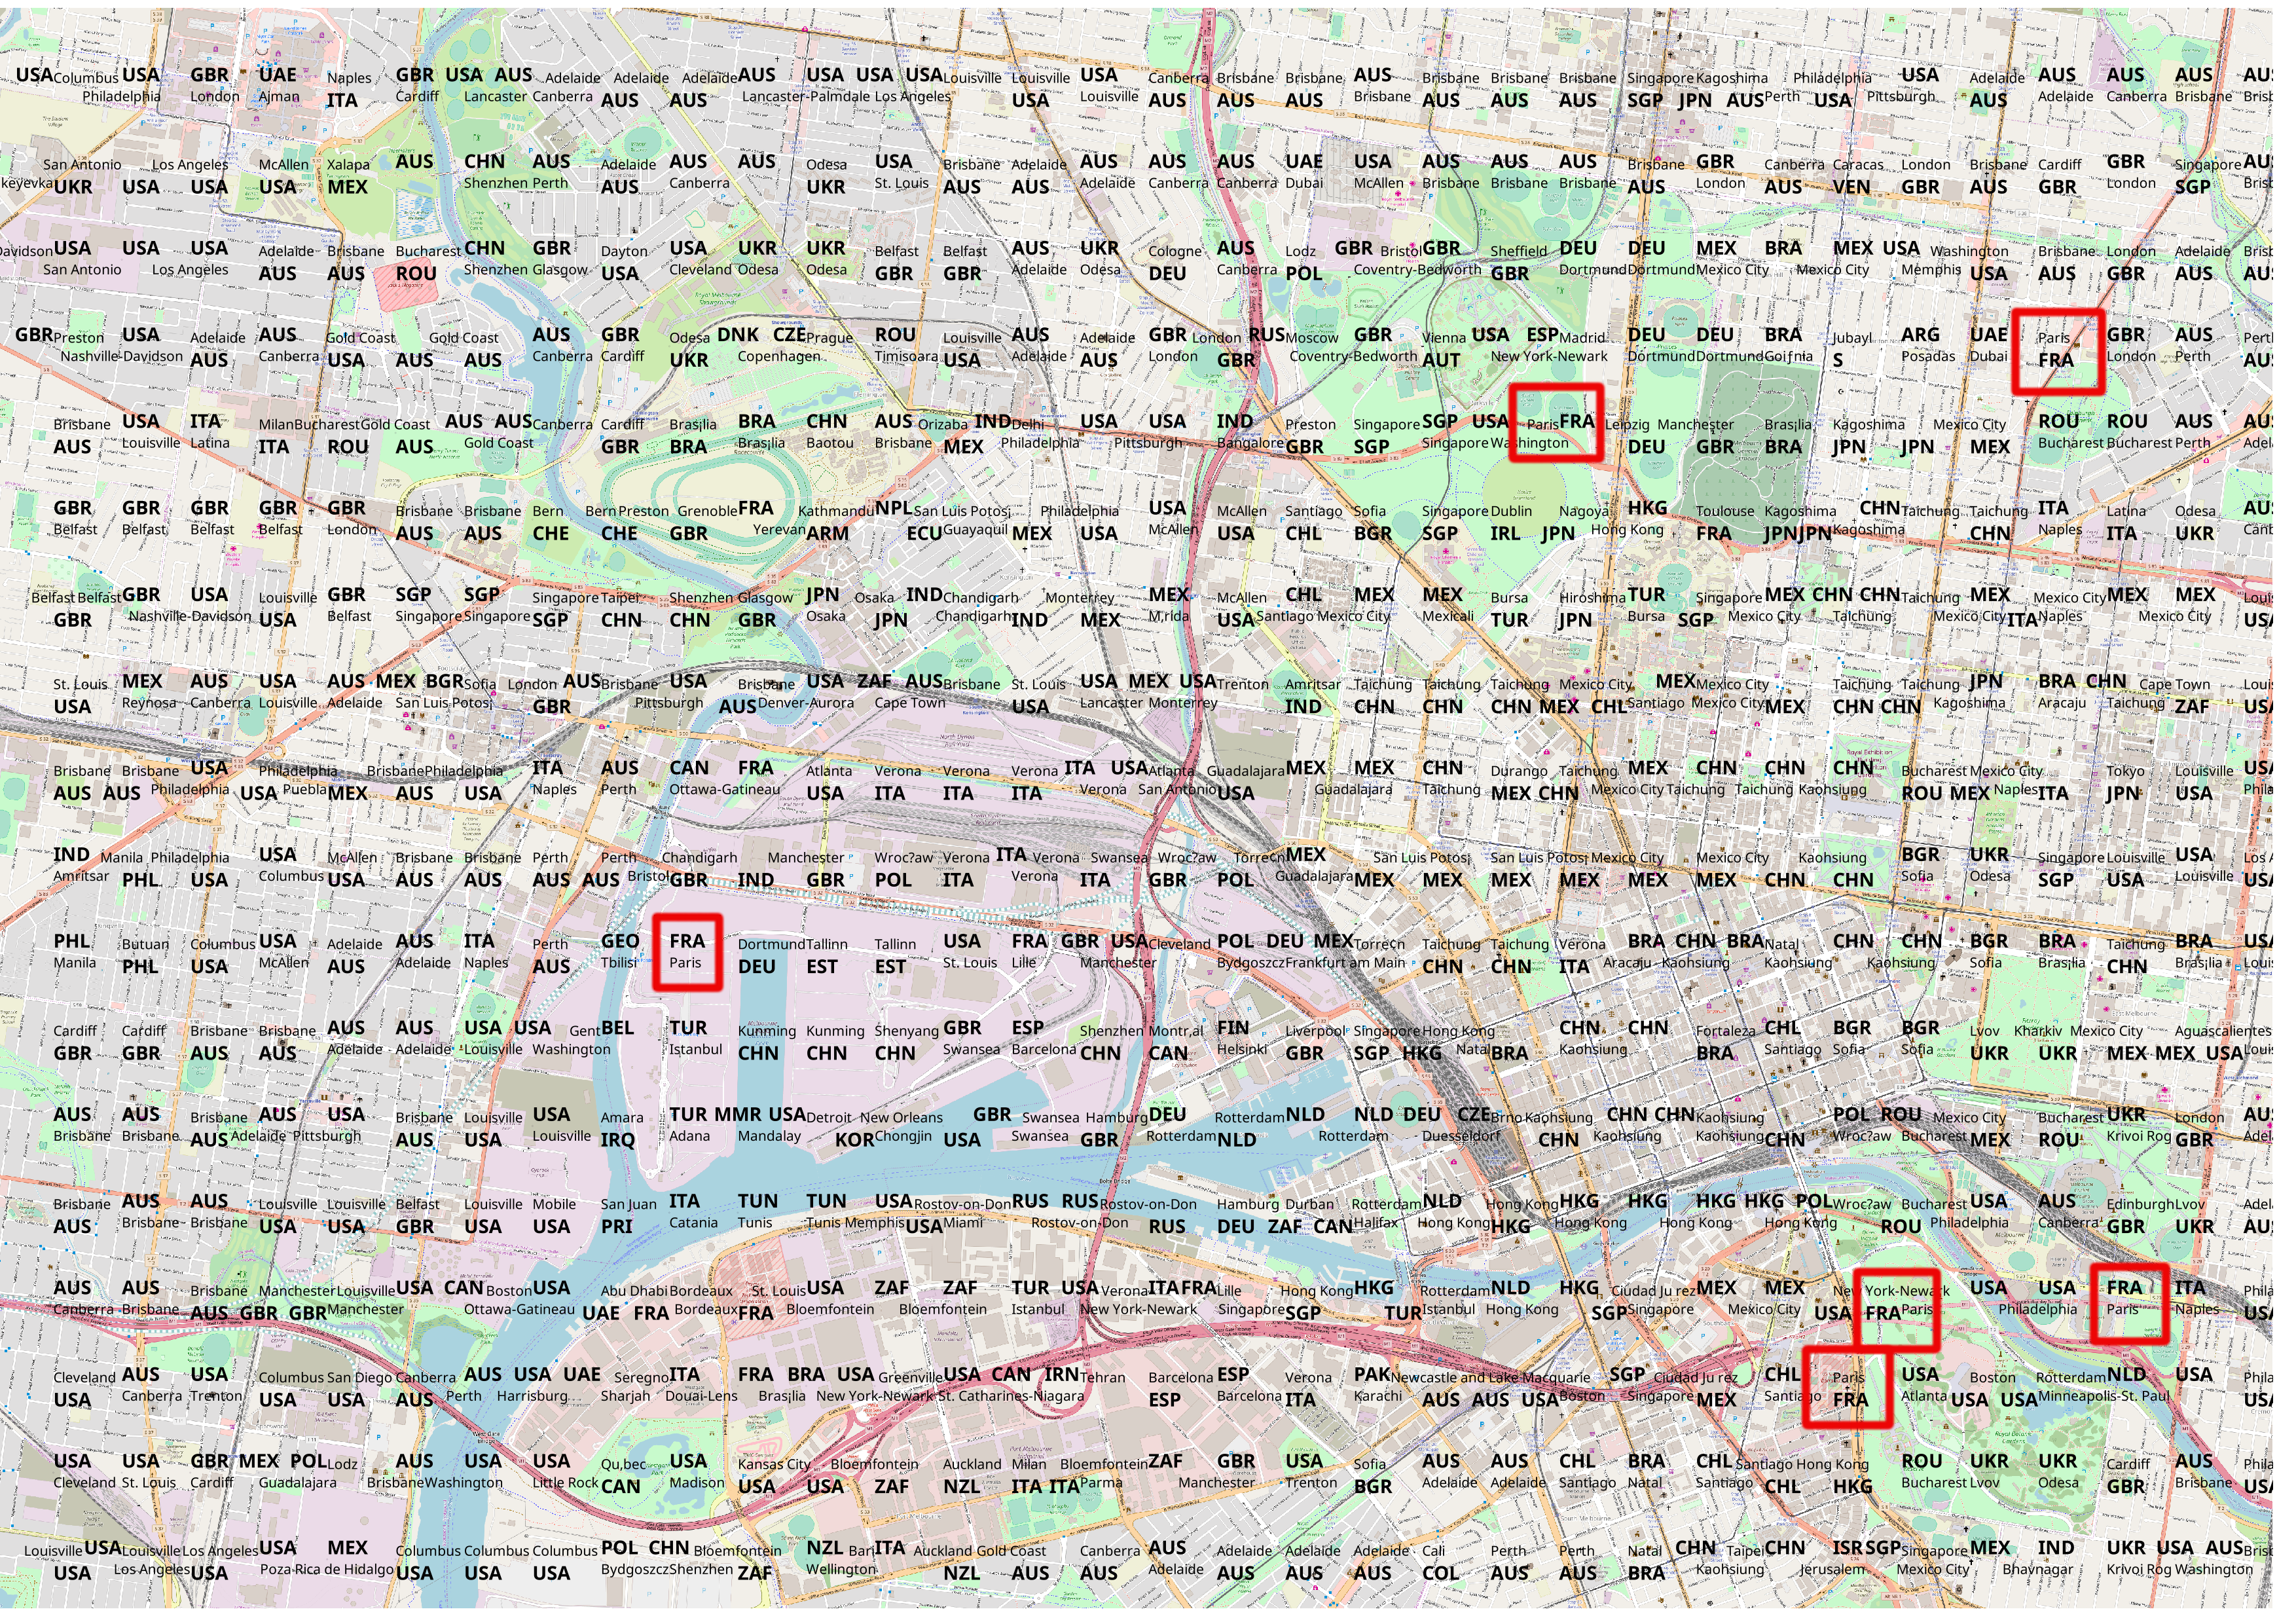
\includegraphics[scale=0.35]{Images/PlosOne/Fig7.png} 
\caption{\bf Predicted similar cities (showing three letter country code of city location) using the GM neural network for Melbourne evaluation locations. Detail of Melbourne CBD, with predictions of Paris highlighted in red squares.}    
 \label{fig:supp_melmapscbd}  
\end{figure} 

\end{document}

